\documentclass[10pt]{article}
\usepackage[T1]{fontenc}
\usepackage{lmodern}
\usepackage{mathtools}
\usepackage{booktabs}
\usepackage{adjustbox}
\usepackage[left=1.5cm, right=2cm, top=1.5cm, bottom=2cm]{geometry}
\usepackage{tikz}
\usepackage{pgfplots}
\pgfplotsset{compat=1.18}
\usetikzlibrary{arrows.meta,positioning,calc}
\setlength\parindent{0pt}
\title{g7 5 - No Protection - Custom Algorithm - Ascending}
\date{}
\author{}

\begin{document}
\maketitle
\section*{Topology}
\begin{center}\begin{adjustbox}{max width=\linewidth}
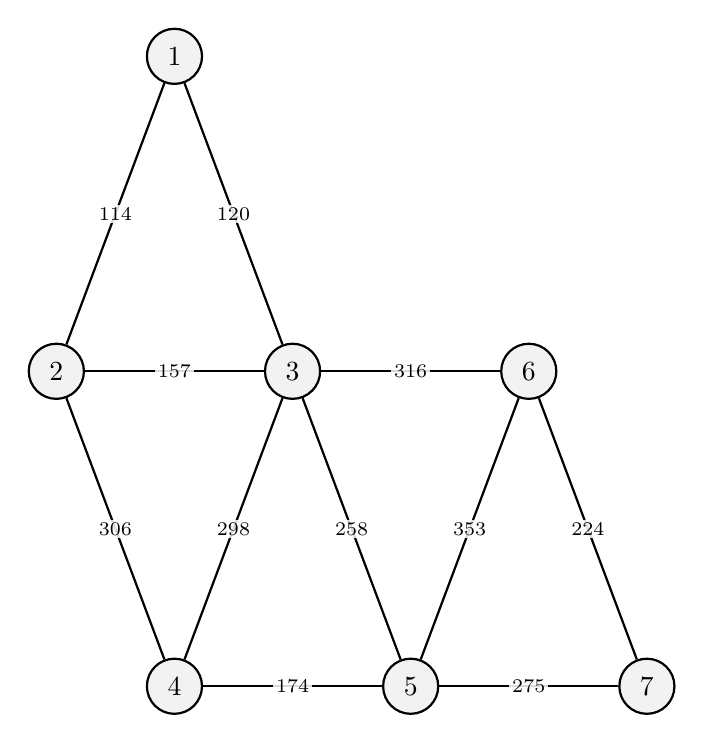
\begin{tikzpicture}[baseline, >={Stealth[length=2mm]},
  netnode/.style={circle, draw, thick, fill=gray!10, minimum size=7mm, inner sep=1pt},
  link/.style={thick},
  linklabel/.style={font=\scriptsize, inner sep=1pt, fill=white, fill opacity=0.85, text opacity=1}]
\node[netnode] (S1) at (1.500,8.000) {1};
\node[netnode] (S2) at (0.000,4.000) {2};
\node[netnode] (S3) at (3.000,4.000) {3};
\node[netnode] (S4) at (1.500,0.000) {4};
\node[netnode] (S5) at (4.500,0.000) {5};
\node[netnode] (S6) at (6.000,4.000) {6};
\node[netnode] (S7) at (7.500,0.000) {7};
\draw[link] (S1) to node[linklabel] {114} (S2);
\draw[link] (S1) to node[linklabel] {120} (S3);
\draw[link] (S2) to node[linklabel] {157} (S3);
\draw[link] (S2) to node[linklabel] {306} (S4);
\draw[link] (S3) to node[linklabel] {298} (S4);
\draw[link] (S3) to node[linklabel] {258} (S5);
\draw[link] (S3) to node[linklabel] {316} (S6);
\draw[link] (S4) to node[linklabel] {174} (S5);
\draw[link] (S5) to node[linklabel] {353} (S6);
\draw[link] (S5) to node[linklabel] {275} (S7);
\draw[link] (S6) to node[linklabel] {224} (S7);
\end{tikzpicture}
\end{adjustbox}\end{center}
\section*{Performance Parameters}
\begin{center}\begin{tabular}{lr}
\toprule
Highest link load & 955 Gb/s \\
Highest used FSU & 194 / 320 \\
Total used FSUs & 231 \\
Transponder cost & 116.0 \\
\midrule
SC-DP-QPSK transponders & 11 \\
SC-DP-16QAM transponders & 22 \\
DP-16QAM transponders & 15 \\
\bottomrule
\end{tabular}\end{center}
\clearpage
\section*{Link Load Map}
\begin{center}\begin{adjustbox}{max width=\linewidth}
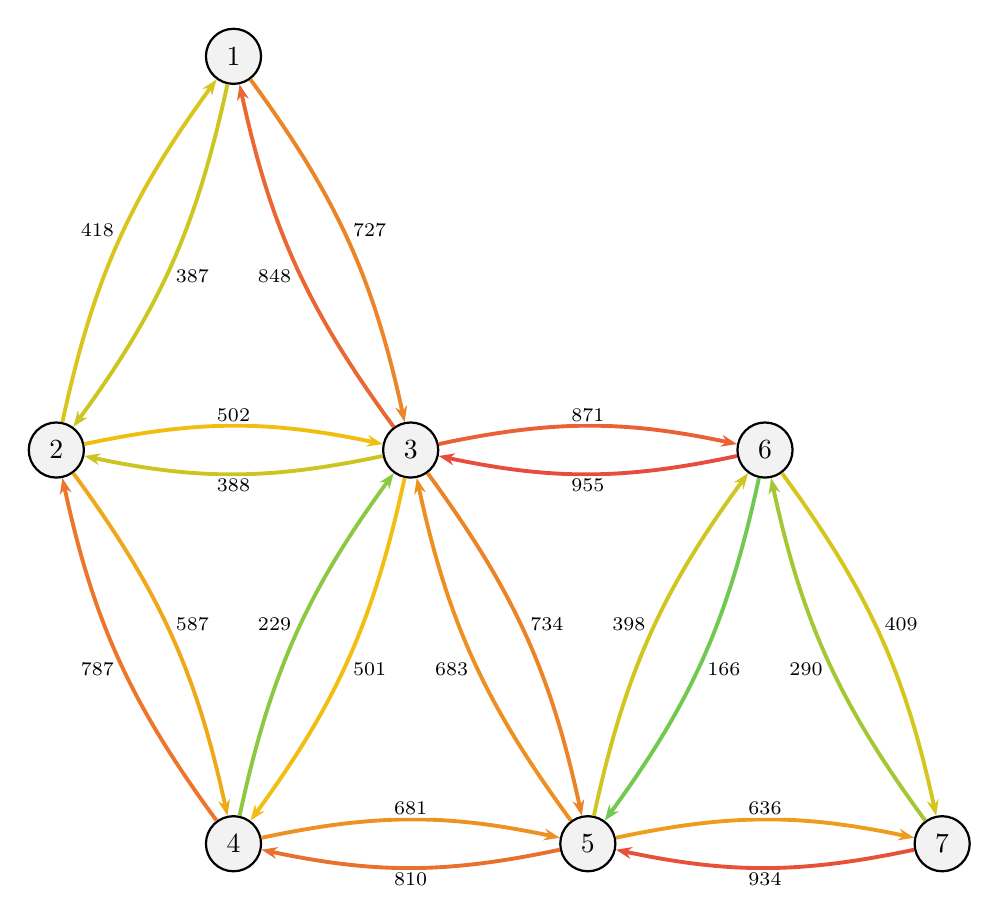
\begin{tikzpicture}[baseline, >={Stealth[length=2mm]},
  netnode/.style={circle, draw, thick, fill=gray!10, minimum size=7mm, inner sep=1pt},
  link/.style={line width=1.4pt},
  linklabel/.style={font=\scriptsize, inner sep=1pt, fill=white, fill opacity=0.85, text opacity=1}]
\node[netnode] (S1) at (2.250,10.000) {1};
\node[netnode] (S2) at (0.000,5.000) {2};
\node[netnode] (S3) at (4.500,5.000) {3};
\node[netnode] (S4) at (2.250,0.000) {4};
\node[netnode] (S5) at (6.750,0.000) {5};
\node[netnode] (S6) at (9.000,5.000) {6};
\node[netnode] (S7) at (11.250,0.000) {7};
\draw[link, ->, draw={rgb,255:red,204;green,198;blue,34}] (S1) to[bend left=12] node[linklabel, auto] {387} (S2);
\draw[link, ->, draw={rgb,255:red,236;green,133;blue,39}] (S1) to[bend left=12] node[linklabel, auto] {727} (S3);
\draw[link, ->, draw={rgb,255:red,217;green,197;blue,27}] (S2) to[bend left=12] node[linklabel, auto] {418} (S1);
\draw[link, ->, draw={rgb,255:red,240;green,190;blue,17}] (S2) to[bend left=12] node[linklabel, auto] {502} (S3);
\draw[link, ->, draw={rgb,255:red,239;green,168;blue,25}] (S2) to[bend left=12] node[linklabel, auto] {587} (S4);
\draw[link, ->, draw={rgb,255:red,233;green,103;blue,50}] (S3) to[bend left=12] node[linklabel, auto] {848} (S1);
\draw[link, ->, draw={rgb,255:red,204;green,197;blue,33}] (S3) to[bend left=12] node[linklabel, auto] {388} (S2);
\draw[link, ->, draw={rgb,255:red,241;green,190;blue,17}] (S3) to[bend left=12] node[linklabel, auto] {501} (S4);
\draw[link, ->, draw={rgb,255:red,236;green,132;blue,39}] (S3) to[bend left=12] node[linklabel, auto] {734} (S5);
\draw[link, ->, draw={rgb,255:red,233;green,97;blue,52}] (S3) to[bend left=12] node[linklabel, auto] {871} (S6);
\draw[link, ->, draw={rgb,255:red,235;green,118;blue,44}] (S4) to[bend left=12] node[linklabel, auto] {787} (S2);
\draw[link, ->, draw={rgb,255:red,140;green,200;blue,66}] (S4) to[bend left=12] node[linklabel, auto] {229} (S3);
\draw[link, ->, draw={rgb,255:red,237;green,145;blue,34}] (S4) to[bend left=12] node[linklabel, auto] {681} (S5);
\draw[link, ->, draw={rgb,255:red,237;green,144;blue,34}] (S5) to[bend left=12] node[linklabel, auto] {683} (S3);
\draw[link, ->, draw={rgb,255:red,234;green,112;blue,46}] (S5) to[bend left=12] node[linklabel, auto] {810} (S4);
\draw[link, ->, draw={rgb,255:red,209;green,197;blue,31}] (S5) to[bend left=12] node[linklabel, auto] {398} (S6);
\draw[link, ->, draw={rgb,255:red,238;green,156;blue,30}] (S5) to[bend left=12] node[linklabel, auto] {636} (S7);
\draw[link, ->, draw={rgb,255:red,231;green,76;blue,60}] (S6) to[bend left=12] node[linklabel, auto] {955} (S3);
\draw[link, ->, draw={rgb,255:red,114;green,201;blue,79}] (S6) to[bend left=12] node[linklabel, auto] {166} (S5);
\draw[link, ->, draw={rgb,255:red,213;green,197;blue,29}] (S6) to[bend left=12] node[linklabel, auto] {409} (S7);
\draw[link, ->, draw={rgb,255:red,231;green,81;blue,58}] (S7) to[bend left=12] node[linklabel, auto] {934} (S5);
\draw[link, ->, draw={rgb,255:red,164;green,199;blue,53}] (S7) to[bend left=12] node[linklabel, auto] {290} (S6);
\end{tikzpicture}
\end{adjustbox}\end{center}
\begin{center}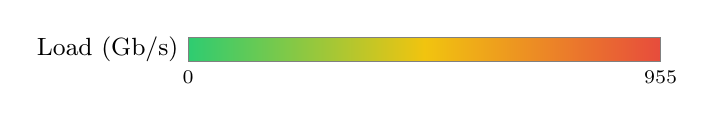
\begin{tikzpicture}
\definecolor{scalelow}{RGB}{46,204,113}\definecolor{scalemid}{RGB}{241,196,15}\definecolor{scalehigh}{RGB}{231,76,60}
\shade[left color=scalelow, right color=scalemid] (0,0) rectangle (3,0.3);
\shade[left color=scalemid, right color=scalehigh] (3,0) rectangle (6,0.3);
\draw[gray] (0,0) rectangle (6,0.3);
\node[below, font=\scriptsize] at (0,0) {0};
\node[below, font=\scriptsize] at (6,0) {955};
\node[left, font=\small] at (0,0.15) {Load (Gb/s)};
\end{tikzpicture}\end{center}
\section*{Link Load Distribution}

\begin{center}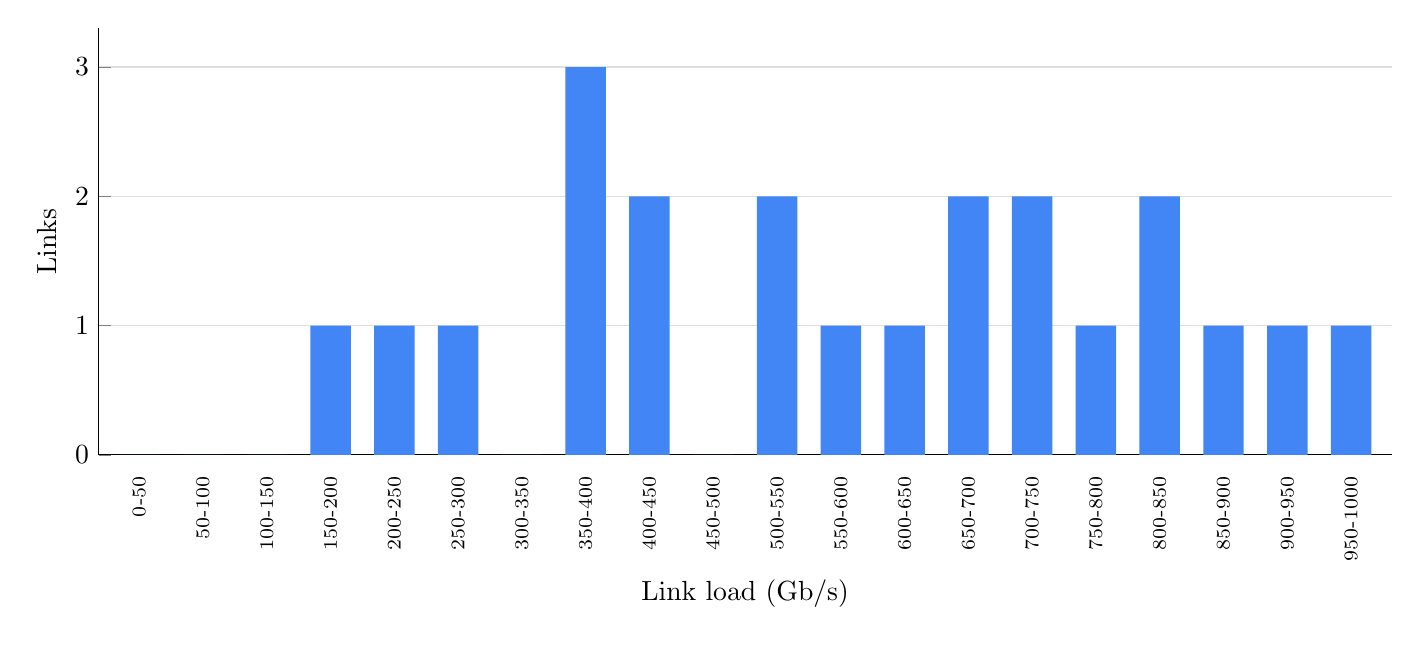
\begin{tikzpicture}
\begin{axis}[
  ybar, bar width=0.514cm, width=18.000cm, height=7cm,
  ymin=0, ymajorgrids, grid style={gray!25}, axis lines*=left,
  enlarge x limits={abs=0.514cm}, xtick=data, major x tick style={draw=none},
  x tick label style={rotate=90, font=\scriptsize, /pgf/number format/1000 sep=},
  legend style={at={(0.5,-0.3)}, anchor=north, legend columns=-1, draw=none},
  ylabel={Links},
  xlabel={Link load (Gb/s)},
  symbolic x coords={0-50,50-100,100-150,150-200,200-250,250-300,300-350,350-400,400-450,450-500,500-550,550-600,600-650,650-700,700-750,750-800,800-850,850-900,900-950,950-1000}]
\addplot[fill={rgb,255:red,66;green,133;blue,244}, draw=none] coordinates {(0-50,0.000) (50-100,0.000) (100-150,0.000) (150-200,1.000) (200-250,1.000) (250-300,1.000) (300-350,0.000) (350-400,3.000) (400-450,2.000) (450-500,0.000) (500-550,2.000) (550-600,1.000) (600-650,1.000) (650-700,2.000) (700-750,2.000) (750-800,1.000) (800-850,2.000) (850-900,1.000) (900-950,1.000) (950-1000,1.000) };
\end{axis}
\end{tikzpicture}\end{center}
\clearpage
\section*{Spectrum Occupancy}
\begin{center}\begin{adjustbox}{max width=\linewidth}
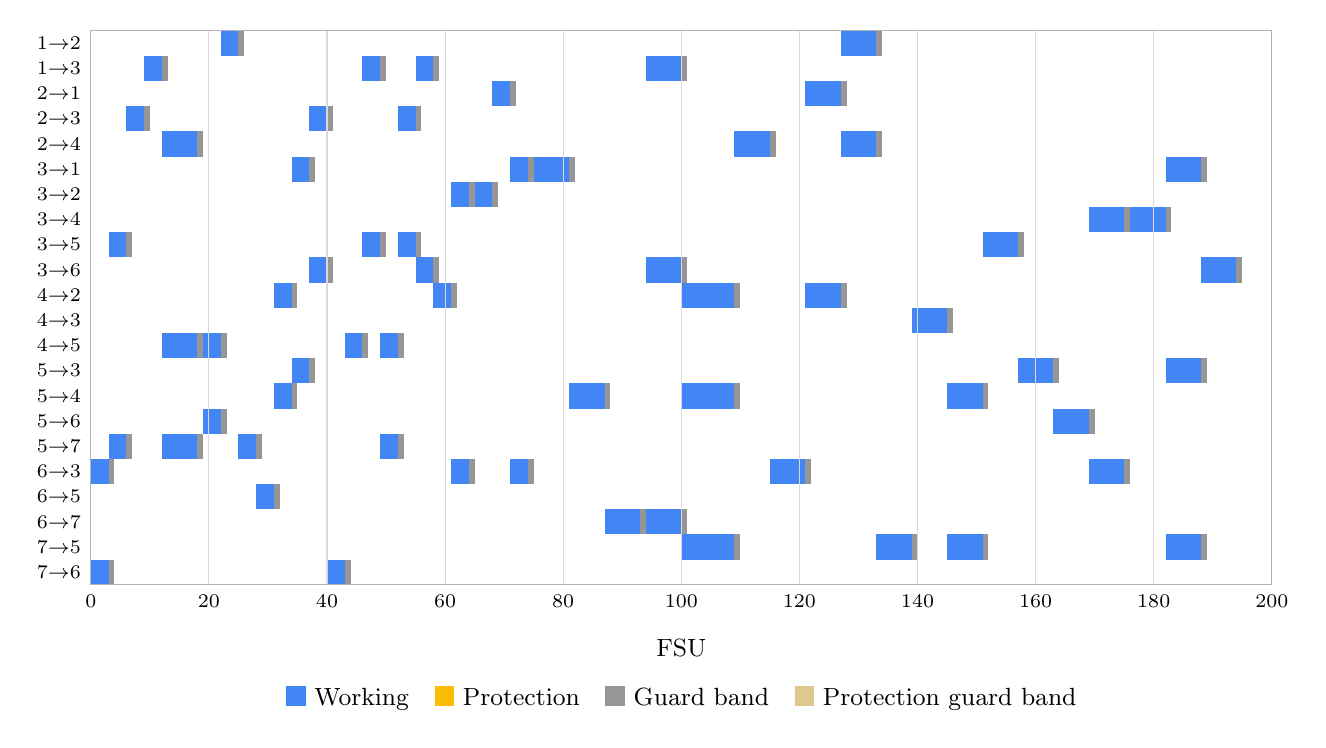
\begin{tikzpicture}[x=0.0750cm, y=-0.32cm]
\fill[fill={rgb,255:red,66;green,133;blue,244}] (22,0) rectangle (25,1);
\fill[fill={rgb,255:red,150;green,150;blue,150}] (25,0) rectangle (26,1);
\fill[fill={rgb,255:red,66;green,133;blue,244}] (127,0) rectangle (133,1);
\fill[fill={rgb,255:red,150;green,150;blue,150}] (133,0) rectangle (134,1);
\node[left, font=\scriptsize] at (0,0.5) {1\(\to\)2};
\fill[fill={rgb,255:red,66;green,133;blue,244}] (9,1) rectangle (12,2);
\fill[fill={rgb,255:red,150;green,150;blue,150}] (12,1) rectangle (13,2);
\fill[fill={rgb,255:red,66;green,133;blue,244}] (46,1) rectangle (49,2);
\fill[fill={rgb,255:red,150;green,150;blue,150}] (49,1) rectangle (50,2);
\fill[fill={rgb,255:red,66;green,133;blue,244}] (55,1) rectangle (58,2);
\fill[fill={rgb,255:red,150;green,150;blue,150}] (58,1) rectangle (59,2);
\fill[fill={rgb,255:red,66;green,133;blue,244}] (94,1) rectangle (100,2);
\fill[fill={rgb,255:red,150;green,150;blue,150}] (100,1) rectangle (101,2);
\node[left, font=\scriptsize] at (0,1.5) {1\(\to\)3};
\fill[fill={rgb,255:red,66;green,133;blue,244}] (68,2) rectangle (71,3);
\fill[fill={rgb,255:red,150;green,150;blue,150}] (71,2) rectangle (72,3);
\fill[fill={rgb,255:red,66;green,133;blue,244}] (121,2) rectangle (127,3);
\fill[fill={rgb,255:red,150;green,150;blue,150}] (127,2) rectangle (128,3);
\node[left, font=\scriptsize] at (0,2.5) {2\(\to\)1};
\fill[fill={rgb,255:red,66;green,133;blue,244}] (6,3) rectangle (9,4);
\fill[fill={rgb,255:red,150;green,150;blue,150}] (9,3) rectangle (10,4);
\fill[fill={rgb,255:red,66;green,133;blue,244}] (37,3) rectangle (40,4);
\fill[fill={rgb,255:red,150;green,150;blue,150}] (40,3) rectangle (41,4);
\fill[fill={rgb,255:red,66;green,133;blue,244}] (52,3) rectangle (55,4);
\fill[fill={rgb,255:red,150;green,150;blue,150}] (55,3) rectangle (56,4);
\node[left, font=\scriptsize] at (0,3.5) {2\(\to\)3};
\fill[fill={rgb,255:red,66;green,133;blue,244}] (12,4) rectangle (18,5);
\fill[fill={rgb,255:red,150;green,150;blue,150}] (18,4) rectangle (19,5);
\fill[fill={rgb,255:red,66;green,133;blue,244}] (109,4) rectangle (115,5);
\fill[fill={rgb,255:red,150;green,150;blue,150}] (115,4) rectangle (116,5);
\fill[fill={rgb,255:red,66;green,133;blue,244}] (127,4) rectangle (133,5);
\fill[fill={rgb,255:red,150;green,150;blue,150}] (133,4) rectangle (134,5);
\node[left, font=\scriptsize] at (0,4.5) {2\(\to\)4};
\fill[fill={rgb,255:red,66;green,133;blue,244}] (34,5) rectangle (37,6);
\fill[fill={rgb,255:red,150;green,150;blue,150}] (37,5) rectangle (38,6);
\fill[fill={rgb,255:red,66;green,133;blue,244}] (71,5) rectangle (74,6);
\fill[fill={rgb,255:red,150;green,150;blue,150}] (74,5) rectangle (75,6);
\fill[fill={rgb,255:red,66;green,133;blue,244}] (75,5) rectangle (81,6);
\fill[fill={rgb,255:red,150;green,150;blue,150}] (81,5) rectangle (82,6);
\fill[fill={rgb,255:red,66;green,133;blue,244}] (182,5) rectangle (188,6);
\fill[fill={rgb,255:red,150;green,150;blue,150}] (188,5) rectangle (189,6);
\node[left, font=\scriptsize] at (0,5.5) {3\(\to\)1};
\fill[fill={rgb,255:red,66;green,133;blue,244}] (61,6) rectangle (64,7);
\fill[fill={rgb,255:red,150;green,150;blue,150}] (64,6) rectangle (65,7);
\fill[fill={rgb,255:red,66;green,133;blue,244}] (65,6) rectangle (68,7);
\fill[fill={rgb,255:red,150;green,150;blue,150}] (68,6) rectangle (69,7);
\node[left, font=\scriptsize] at (0,6.5) {3\(\to\)2};
\fill[fill={rgb,255:red,66;green,133;blue,244}] (169,7) rectangle (175,8);
\fill[fill={rgb,255:red,150;green,150;blue,150}] (175,7) rectangle (176,8);
\fill[fill={rgb,255:red,66;green,133;blue,244}] (176,7) rectangle (182,8);
\fill[fill={rgb,255:red,150;green,150;blue,150}] (182,7) rectangle (183,8);
\node[left, font=\scriptsize] at (0,7.5) {3\(\to\)4};
\fill[fill={rgb,255:red,66;green,133;blue,244}] (3,8) rectangle (6,9);
\fill[fill={rgb,255:red,150;green,150;blue,150}] (6,8) rectangle (7,9);
\fill[fill={rgb,255:red,66;green,133;blue,244}] (46,8) rectangle (49,9);
\fill[fill={rgb,255:red,150;green,150;blue,150}] (49,8) rectangle (50,9);
\fill[fill={rgb,255:red,66;green,133;blue,244}] (52,8) rectangle (55,9);
\fill[fill={rgb,255:red,150;green,150;blue,150}] (55,8) rectangle (56,9);
\fill[fill={rgb,255:red,66;green,133;blue,244}] (151,8) rectangle (157,9);
\fill[fill={rgb,255:red,150;green,150;blue,150}] (157,8) rectangle (158,9);
\node[left, font=\scriptsize] at (0,8.5) {3\(\to\)5};
\fill[fill={rgb,255:red,66;green,133;blue,244}] (37,9) rectangle (40,10);
\fill[fill={rgb,255:red,150;green,150;blue,150}] (40,9) rectangle (41,10);
\fill[fill={rgb,255:red,66;green,133;blue,244}] (55,9) rectangle (58,10);
\fill[fill={rgb,255:red,150;green,150;blue,150}] (58,9) rectangle (59,10);
\fill[fill={rgb,255:red,66;green,133;blue,244}] (94,9) rectangle (100,10);
\fill[fill={rgb,255:red,150;green,150;blue,150}] (100,9) rectangle (101,10);
\fill[fill={rgb,255:red,66;green,133;blue,244}] (188,9) rectangle (194,10);
\fill[fill={rgb,255:red,150;green,150;blue,150}] (194,9) rectangle (195,10);
\node[left, font=\scriptsize] at (0,9.5) {3\(\to\)6};
\fill[fill={rgb,255:red,66;green,133;blue,244}] (31,10) rectangle (34,11);
\fill[fill={rgb,255:red,150;green,150;blue,150}] (34,10) rectangle (35,11);
\fill[fill={rgb,255:red,66;green,133;blue,244}] (58,10) rectangle (61,11);
\fill[fill={rgb,255:red,150;green,150;blue,150}] (61,10) rectangle (62,11);
\fill[fill={rgb,255:red,66;green,133;blue,244}] (100,10) rectangle (109,11);
\fill[fill={rgb,255:red,150;green,150;blue,150}] (109,10) rectangle (110,11);
\fill[fill={rgb,255:red,66;green,133;blue,244}] (121,10) rectangle (127,11);
\fill[fill={rgb,255:red,150;green,150;blue,150}] (127,10) rectangle (128,11);
\node[left, font=\scriptsize] at (0,10.5) {4\(\to\)2};
\fill[fill={rgb,255:red,66;green,133;blue,244}] (139,11) rectangle (145,12);
\fill[fill={rgb,255:red,150;green,150;blue,150}] (145,11) rectangle (146,12);
\node[left, font=\scriptsize] at (0,11.5) {4\(\to\)3};
\fill[fill={rgb,255:red,66;green,133;blue,244}] (12,12) rectangle (18,13);
\fill[fill={rgb,255:red,150;green,150;blue,150}] (18,12) rectangle (19,13);
\fill[fill={rgb,255:red,66;green,133;blue,244}] (19,12) rectangle (22,13);
\fill[fill={rgb,255:red,150;green,150;blue,150}] (22,12) rectangle (23,13);
\fill[fill={rgb,255:red,66;green,133;blue,244}] (43,12) rectangle (46,13);
\fill[fill={rgb,255:red,150;green,150;blue,150}] (46,12) rectangle (47,13);
\fill[fill={rgb,255:red,66;green,133;blue,244}] (49,12) rectangle (52,13);
\fill[fill={rgb,255:red,150;green,150;blue,150}] (52,12) rectangle (53,13);
\node[left, font=\scriptsize] at (0,12.5) {4\(\to\)5};
\fill[fill={rgb,255:red,66;green,133;blue,244}] (34,13) rectangle (37,14);
\fill[fill={rgb,255:red,150;green,150;blue,150}] (37,13) rectangle (38,14);
\fill[fill={rgb,255:red,66;green,133;blue,244}] (157,13) rectangle (163,14);
\fill[fill={rgb,255:red,150;green,150;blue,150}] (163,13) rectangle (164,14);
\fill[fill={rgb,255:red,66;green,133;blue,244}] (182,13) rectangle (188,14);
\fill[fill={rgb,255:red,150;green,150;blue,150}] (188,13) rectangle (189,14);
\node[left, font=\scriptsize] at (0,13.5) {5\(\to\)3};
\fill[fill={rgb,255:red,66;green,133;blue,244}] (31,14) rectangle (34,15);
\fill[fill={rgb,255:red,150;green,150;blue,150}] (34,14) rectangle (35,15);
\fill[fill={rgb,255:red,66;green,133;blue,244}] (81,14) rectangle (87,15);
\fill[fill={rgb,255:red,150;green,150;blue,150}] (87,14) rectangle (88,15);
\fill[fill={rgb,255:red,66;green,133;blue,244}] (100,14) rectangle (109,15);
\fill[fill={rgb,255:red,150;green,150;blue,150}] (109,14) rectangle (110,15);
\fill[fill={rgb,255:red,66;green,133;blue,244}] (145,14) rectangle (151,15);
\fill[fill={rgb,255:red,150;green,150;blue,150}] (151,14) rectangle (152,15);
\node[left, font=\scriptsize] at (0,14.5) {5\(\to\)4};
\fill[fill={rgb,255:red,66;green,133;blue,244}] (19,15) rectangle (22,16);
\fill[fill={rgb,255:red,150;green,150;blue,150}] (22,15) rectangle (23,16);
\fill[fill={rgb,255:red,66;green,133;blue,244}] (163,15) rectangle (169,16);
\fill[fill={rgb,255:red,150;green,150;blue,150}] (169,15) rectangle (170,16);
\node[left, font=\scriptsize] at (0,15.5) {5\(\to\)6};
\fill[fill={rgb,255:red,66;green,133;blue,244}] (3,16) rectangle (6,17);
\fill[fill={rgb,255:red,150;green,150;blue,150}] (6,16) rectangle (7,17);
\fill[fill={rgb,255:red,66;green,133;blue,244}] (12,16) rectangle (18,17);
\fill[fill={rgb,255:red,150;green,150;blue,150}] (18,16) rectangle (19,17);
\fill[fill={rgb,255:red,66;green,133;blue,244}] (25,16) rectangle (28,17);
\fill[fill={rgb,255:red,150;green,150;blue,150}] (28,16) rectangle (29,17);
\fill[fill={rgb,255:red,66;green,133;blue,244}] (49,16) rectangle (52,17);
\fill[fill={rgb,255:red,150;green,150;blue,150}] (52,16) rectangle (53,17);
\node[left, font=\scriptsize] at (0,16.5) {5\(\to\)7};
\fill[fill={rgb,255:red,66;green,133;blue,244}] (0,17) rectangle (3,18);
\fill[fill={rgb,255:red,150;green,150;blue,150}] (3,17) rectangle (4,18);
\fill[fill={rgb,255:red,66;green,133;blue,244}] (61,17) rectangle (64,18);
\fill[fill={rgb,255:red,150;green,150;blue,150}] (64,17) rectangle (65,18);
\fill[fill={rgb,255:red,66;green,133;blue,244}] (71,17) rectangle (74,18);
\fill[fill={rgb,255:red,150;green,150;blue,150}] (74,17) rectangle (75,18);
\fill[fill={rgb,255:red,66;green,133;blue,244}] (115,17) rectangle (121,18);
\fill[fill={rgb,255:red,150;green,150;blue,150}] (121,17) rectangle (122,18);
\fill[fill={rgb,255:red,66;green,133;blue,244}] (169,17) rectangle (175,18);
\fill[fill={rgb,255:red,150;green,150;blue,150}] (175,17) rectangle (176,18);
\node[left, font=\scriptsize] at (0,17.5) {6\(\to\)3};
\fill[fill={rgb,255:red,66;green,133;blue,244}] (28,18) rectangle (31,19);
\fill[fill={rgb,255:red,150;green,150;blue,150}] (31,18) rectangle (32,19);
\node[left, font=\scriptsize] at (0,18.5) {6\(\to\)5};
\fill[fill={rgb,255:red,66;green,133;blue,244}] (87,19) rectangle (93,20);
\fill[fill={rgb,255:red,150;green,150;blue,150}] (93,19) rectangle (94,20);
\fill[fill={rgb,255:red,66;green,133;blue,244}] (94,19) rectangle (100,20);
\fill[fill={rgb,255:red,150;green,150;blue,150}] (100,19) rectangle (101,20);
\node[left, font=\scriptsize] at (0,19.5) {6\(\to\)7};
\fill[fill={rgb,255:red,66;green,133;blue,244}] (100,20) rectangle (109,21);
\fill[fill={rgb,255:red,150;green,150;blue,150}] (109,20) rectangle (110,21);
\fill[fill={rgb,255:red,66;green,133;blue,244}] (133,20) rectangle (139,21);
\fill[fill={rgb,255:red,150;green,150;blue,150}] (139,20) rectangle (140,21);
\fill[fill={rgb,255:red,66;green,133;blue,244}] (145,20) rectangle (151,21);
\fill[fill={rgb,255:red,150;green,150;blue,150}] (151,20) rectangle (152,21);
\fill[fill={rgb,255:red,66;green,133;blue,244}] (182,20) rectangle (188,21);
\fill[fill={rgb,255:red,150;green,150;blue,150}] (188,20) rectangle (189,21);
\node[left, font=\scriptsize] at (0,20.5) {7\(\to\)5};
\fill[fill={rgb,255:red,66;green,133;blue,244}] (0,21) rectangle (3,22);
\fill[fill={rgb,255:red,150;green,150;blue,150}] (3,21) rectangle (4,22);
\fill[fill={rgb,255:red,66;green,133;blue,244}] (40,21) rectangle (43,22);
\fill[fill={rgb,255:red,150;green,150;blue,150}] (43,21) rectangle (44,22);
\node[left, font=\scriptsize] at (0,21.5) {7\(\to\)6};
\foreach \s in {0,20,...,200} {\draw[gray!30] (\s,0) -- (\s,22); \node[below, font=\scriptsize] at (\s,22) {\s};}
\draw[gray!60] (0,0) rectangle (200,22);
\node[font=\small] at (100.0,24.5) {FSU};
\node[font=\small] at (100.0,26.5) {\textcolor[RGB]{66,133,244}{\rule{2.5mm}{2.5mm}} Working\quad \textcolor[RGB]{251,188,5}{\rule{2.5mm}{2.5mm}} Protection\quad \textcolor[RGB]{150,150,150}{\rule{2.5mm}{2.5mm}} Guard band\quad \textcolor[RGB]{222,200,140}{\rule{2.5mm}{2.5mm}} Protection guard band\quad };
\end{tikzpicture}
\end{adjustbox}\end{center}
\clearpage
\section*{Path Length Distribution}

\begin{center}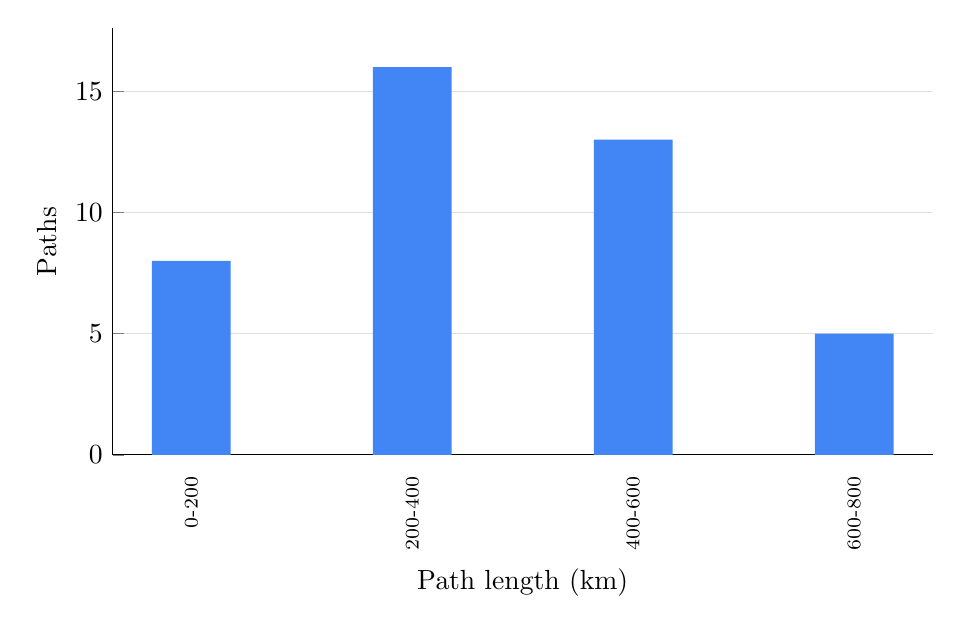
\begin{tikzpicture}
\begin{axis}[
  ybar, bar width=1.000cm, width=12.000cm, height=7cm,
  ymin=0, ymajorgrids, grid style={gray!25}, axis lines*=left,
  enlarge x limits={abs=1.000cm}, xtick=data, major x tick style={draw=none},
  x tick label style={rotate=90, font=\scriptsize, /pgf/number format/1000 sep=},
  legend style={at={(0.5,-0.3)}, anchor=north, legend columns=-1, draw=none},
  ylabel={Paths},
  xlabel={Path length (km)},
  symbolic x coords={0-200,200-400,400-600,600-800,800-1000,1000-1200,1200-1400,1400-1600,1600-1800,1800-2000}]
\addplot[fill={rgb,255:red,66;green,133;blue,244}, draw=none] coordinates {(0-200,8.000) (200-400,16.000) (400-600,13.000) (600-800,5.000) };
\end{axis}
\end{tikzpicture}\end{center}
\clearpage
\section*{Utilization Entropy}
\begin{center}\begin{adjustbox}{max width=\linewidth}
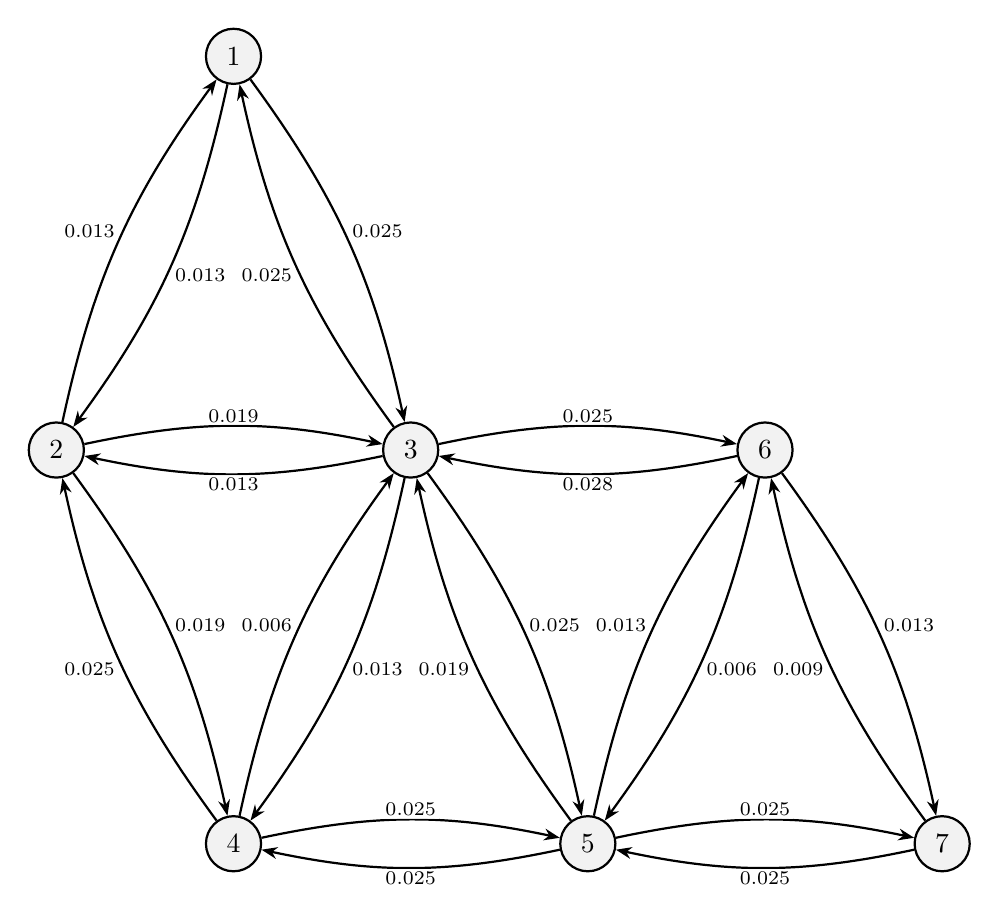
\begin{tikzpicture}[baseline, >={Stealth[length=2mm]},
  netnode/.style={circle, draw, thick, fill=gray!10, minimum size=7mm, inner sep=1pt},
  link/.style={thick},
  linklabel/.style={font=\scriptsize, inner sep=1pt, fill=white, fill opacity=0.85, text opacity=1}]
\node[netnode] (S1) at (2.250,10.000) {1};
\node[netnode] (S2) at (0.000,5.000) {2};
\node[netnode] (S3) at (4.500,5.000) {3};
\node[netnode] (S4) at (2.250,0.000) {4};
\node[netnode] (S5) at (6.750,0.000) {5};
\node[netnode] (S6) at (9.000,5.000) {6};
\node[netnode] (S7) at (11.250,0.000) {7};
\draw[link, ->] (S1) to[bend left=12] node[linklabel, auto] {0.013} (S2);
\draw[link, ->] (S1) to[bend left=12] node[linklabel, auto] {0.025} (S3);
\draw[link, ->] (S2) to[bend left=12] node[linklabel, auto] {0.013} (S1);
\draw[link, ->] (S2) to[bend left=12] node[linklabel, auto] {0.019} (S3);
\draw[link, ->] (S2) to[bend left=12] node[linklabel, auto] {0.019} (S4);
\draw[link, ->] (S3) to[bend left=12] node[linklabel, auto] {0.025} (S1);
\draw[link, ->] (S3) to[bend left=12] node[linklabel, auto] {0.013} (S2);
\draw[link, ->] (S3) to[bend left=12] node[linklabel, auto] {0.013} (S4);
\draw[link, ->] (S3) to[bend left=12] node[linklabel, auto] {0.025} (S5);
\draw[link, ->] (S3) to[bend left=12] node[linklabel, auto] {0.025} (S6);
\draw[link, ->] (S4) to[bend left=12] node[linklabel, auto] {0.025} (S2);
\draw[link, ->] (S4) to[bend left=12] node[linklabel, auto] {0.006} (S3);
\draw[link, ->] (S4) to[bend left=12] node[linklabel, auto] {0.025} (S5);
\draw[link, ->] (S5) to[bend left=12] node[linklabel, auto] {0.019} (S3);
\draw[link, ->] (S5) to[bend left=12] node[linklabel, auto] {0.025} (S4);
\draw[link, ->] (S5) to[bend left=12] node[linklabel, auto] {0.013} (S6);
\draw[link, ->] (S5) to[bend left=12] node[linklabel, auto] {0.025} (S7);
\draw[link, ->] (S6) to[bend left=12] node[linklabel, auto] {0.028} (S3);
\draw[link, ->] (S6) to[bend left=12] node[linklabel, auto] {0.006} (S5);
\draw[link, ->] (S6) to[bend left=12] node[linklabel, auto] {0.013} (S7);
\draw[link, ->] (S7) to[bend left=12] node[linklabel, auto] {0.025} (S5);
\draw[link, ->] (S7) to[bend left=12] node[linklabel, auto] {0.009} (S6);
\end{tikzpicture}
\end{adjustbox}\end{center}

\begin{center}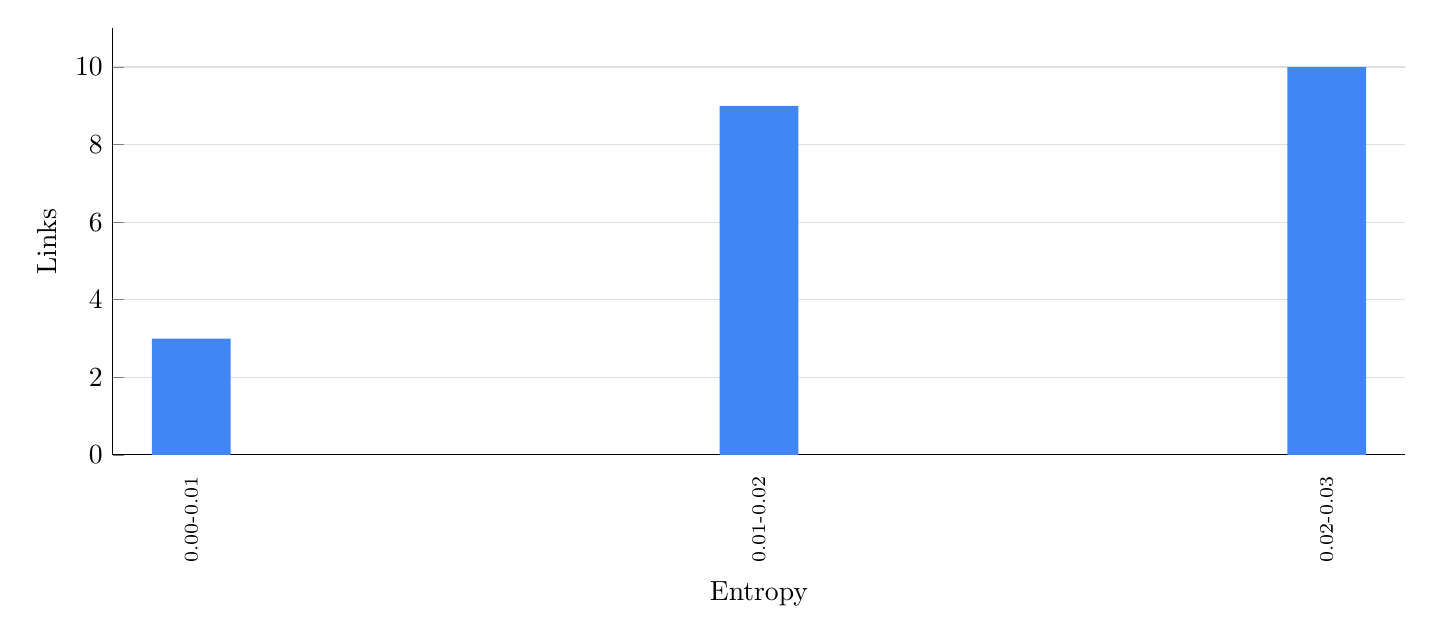
\begin{tikzpicture}
\begin{axis}[
  ybar, bar width=1.000cm, width=18.000cm, height=7cm,
  ymin=0, ymajorgrids, grid style={gray!25}, axis lines*=left,
  enlarge x limits={abs=1.000cm}, xtick=data, major x tick style={draw=none},
  x tick label style={rotate=90, font=\scriptsize, /pgf/number format/1000 sep=},
  legend style={at={(0.5,-0.3)}, anchor=north, legend columns=-1, draw=none},
  ylabel={Links},
  xlabel={Entropy},
  symbolic x coords={0.00-0.01,0.01-0.02,0.02-0.03,0.03-0.04,0.04-0.05,0.05-0.06,0.06-0.07,0.07-0.08,0.08-0.09,0.09-0.10,0.10-0.11,0.11-0.12,0.12-0.13,0.13-0.14,0.14-0.15,0.15-0.16,0.16-0.17,0.17-0.18,0.18-0.19,0.19-0.20,0.20-0.21,0.21-0.22,0.22-0.23,0.23-0.24,0.24-0.25,0.25-0.26,0.26-0.27,0.27-0.28,0.28-0.29,0.29-0.30,0.30-0.31,0.31-0.32,0.32-0.33,0.33-0.34,0.34-0.35,0.35-0.36,0.36-0.37,0.37-0.38,0.38-0.39,0.39-0.40,0.40-0.41,0.41-0.42,0.42-0.43,0.43-0.44,0.44-0.45,0.45-0.46,0.46-0.47,0.47-0.48,0.48-0.49,0.49-0.50,0.50-0.51,0.51-0.52,0.52-0.53,0.53-0.54,0.54-0.55,0.55-0.56,0.56-0.57,0.57-0.58,0.58-0.59,0.59-0.60,0.60-0.61,0.61-0.62,0.62-0.63,0.63-0.64,0.64-0.65,0.65-0.66,0.66-0.67,0.67-0.68,0.68-0.69,0.69-0.70,0.70-0.71,0.71-0.72,0.72-0.73,0.73-0.74,0.74-0.75,0.75-0.76,0.76-0.77,0.77-0.78,0.78-0.79,0.79-0.80,0.80-0.81,0.81-0.82,0.82-0.83,0.83-0.84,0.84-0.85,0.85-0.86,0.86-0.87,0.87-0.88,0.88-0.89,0.89-0.90,0.90-0.91,0.91-0.92,0.92-0.93,0.93-0.94,0.94-0.95,0.95-0.96,0.96-0.97,0.97-0.98,0.98-0.99,0.99-1.00}]
\addplot[fill={rgb,255:red,66;green,133;blue,244}, draw=none] coordinates {(0.00-0.01,3.000) (0.01-0.02,9.000) (0.02-0.03,10.000) };
\end{axis}
\end{tikzpicture}\end{center}
\clearpage
\section*{Shannon Entropy}
\begin{center}\begin{adjustbox}{max width=\linewidth}
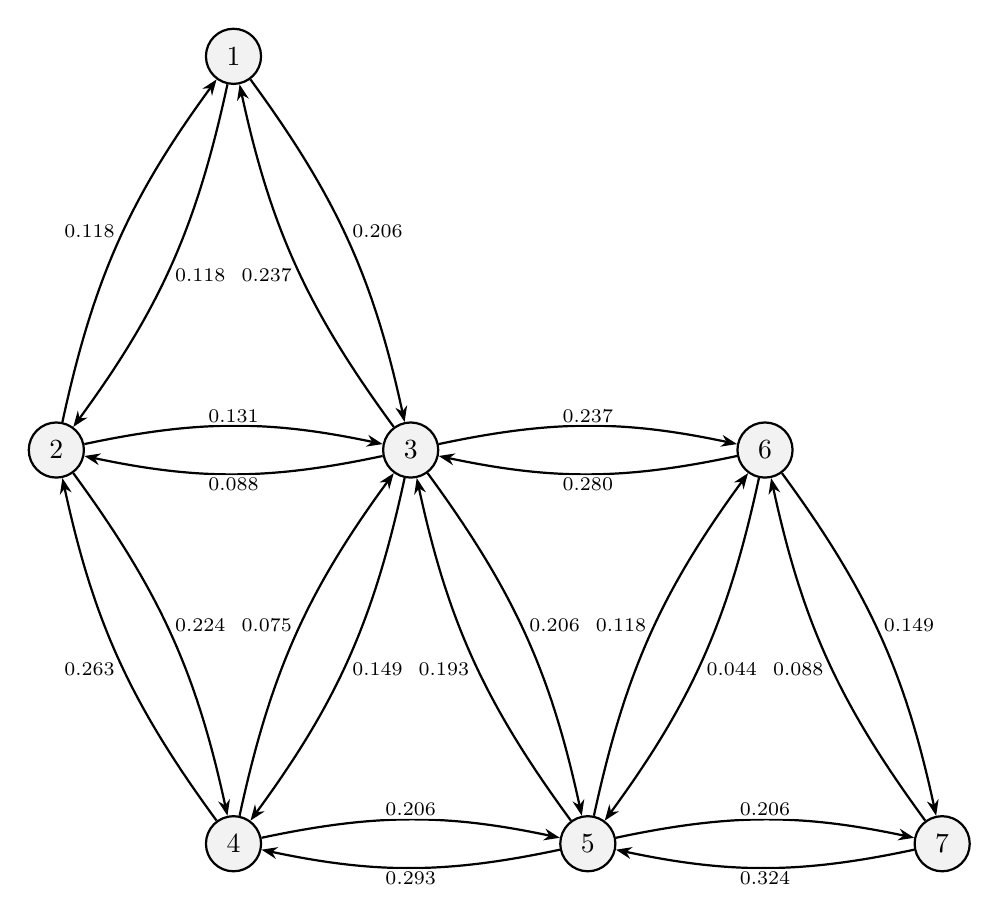
\begin{tikzpicture}[baseline, >={Stealth[length=2mm]},
  netnode/.style={circle, draw, thick, fill=gray!10, minimum size=7mm, inner sep=1pt},
  link/.style={thick},
  linklabel/.style={font=\scriptsize, inner sep=1pt, fill=white, fill opacity=0.85, text opacity=1}]
\node[netnode] (S1) at (2.250,10.000) {1};
\node[netnode] (S2) at (0.000,5.000) {2};
\node[netnode] (S3) at (4.500,5.000) {3};
\node[netnode] (S4) at (2.250,0.000) {4};
\node[netnode] (S5) at (6.750,0.000) {5};
\node[netnode] (S6) at (9.000,5.000) {6};
\node[netnode] (S7) at (11.250,0.000) {7};
\draw[link, ->] (S1) to[bend left=12] node[linklabel, auto] {0.118} (S2);
\draw[link, ->] (S1) to[bend left=12] node[linklabel, auto] {0.206} (S3);
\draw[link, ->] (S2) to[bend left=12] node[linklabel, auto] {0.118} (S1);
\draw[link, ->] (S2) to[bend left=12] node[linklabel, auto] {0.131} (S3);
\draw[link, ->] (S2) to[bend left=12] node[linklabel, auto] {0.224} (S4);
\draw[link, ->] (S3) to[bend left=12] node[linklabel, auto] {0.237} (S1);
\draw[link, ->] (S3) to[bend left=12] node[linklabel, auto] {0.088} (S2);
\draw[link, ->] (S3) to[bend left=12] node[linklabel, auto] {0.149} (S4);
\draw[link, ->] (S3) to[bend left=12] node[linklabel, auto] {0.206} (S5);
\draw[link, ->] (S3) to[bend left=12] node[linklabel, auto] {0.237} (S6);
\draw[link, ->] (S4) to[bend left=12] node[linklabel, auto] {0.263} (S2);
\draw[link, ->] (S4) to[bend left=12] node[linklabel, auto] {0.075} (S3);
\draw[link, ->] (S4) to[bend left=12] node[linklabel, auto] {0.206} (S5);
\draw[link, ->] (S5) to[bend left=12] node[linklabel, auto] {0.193} (S3);
\draw[link, ->] (S5) to[bend left=12] node[linklabel, auto] {0.293} (S4);
\draw[link, ->] (S5) to[bend left=12] node[linklabel, auto] {0.118} (S6);
\draw[link, ->] (S5) to[bend left=12] node[linklabel, auto] {0.206} (S7);
\draw[link, ->] (S6) to[bend left=12] node[linklabel, auto] {0.280} (S3);
\draw[link, ->] (S6) to[bend left=12] node[linklabel, auto] {0.044} (S5);
\draw[link, ->] (S6) to[bend left=12] node[linklabel, auto] {0.149} (S7);
\draw[link, ->] (S7) to[bend left=12] node[linklabel, auto] {0.324} (S5);
\draw[link, ->] (S7) to[bend left=12] node[linklabel, auto] {0.088} (S6);
\end{tikzpicture}
\end{adjustbox}\end{center}

\begin{center}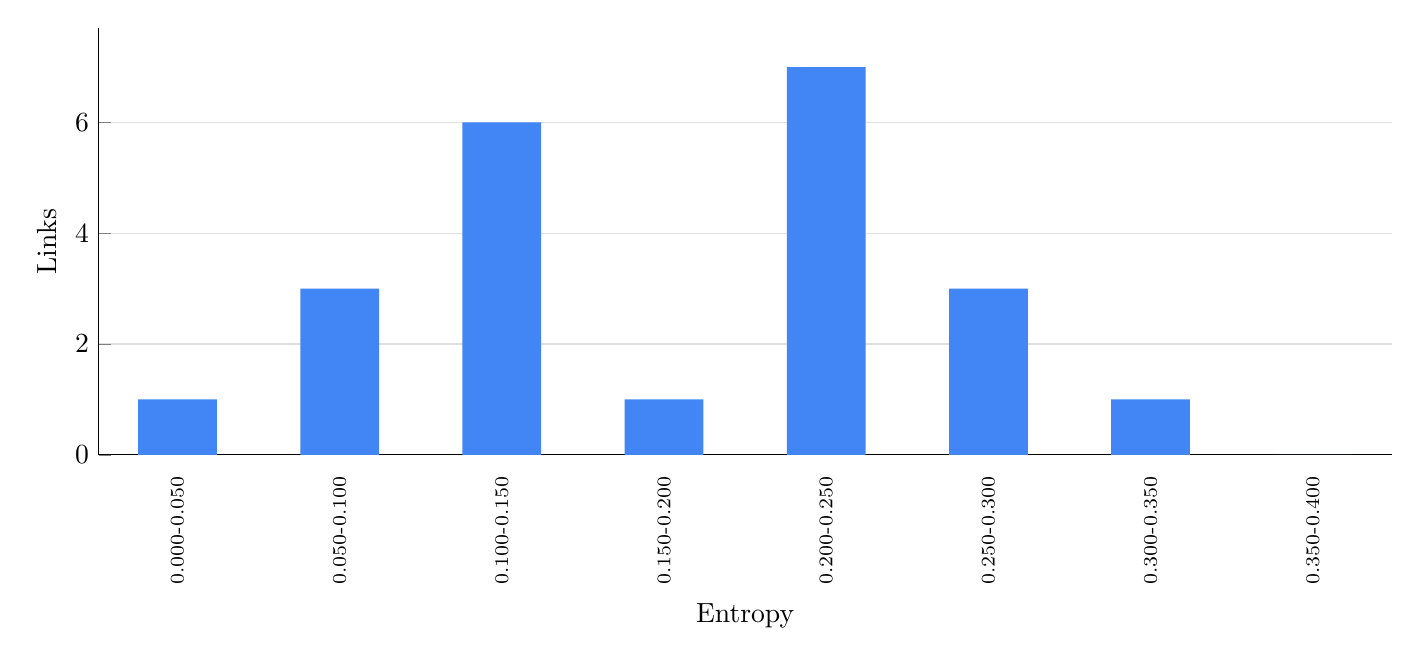
\begin{tikzpicture}
\begin{axis}[
  ybar, bar width=1.000cm, width=18.000cm, height=7cm,
  ymin=0, ymajorgrids, grid style={gray!25}, axis lines*=left,
  enlarge x limits={abs=1.000cm}, xtick=data, major x tick style={draw=none},
  x tick label style={rotate=90, font=\scriptsize, /pgf/number format/1000 sep=},
  legend style={at={(0.5,-0.3)}, anchor=north, legend columns=-1, draw=none},
  ylabel={Links},
  xlabel={Entropy},
  symbolic x coords={0.000-0.050,0.050-0.100,0.100-0.150,0.150-0.200,0.200-0.250,0.250-0.300,0.300-0.350,0.350-0.400,0.400-0.450,0.450-0.500,0.500-0.550,0.550-0.600,0.600-0.650,0.650-0.700,0.700-0.750,0.750-0.800,0.800-0.850,0.850-0.900,0.900-0.950,0.950-1.000}]
\addplot[fill={rgb,255:red,66;green,133;blue,244}, draw=none] coordinates {(0.000-0.050,1.000) (0.050-0.100,3.000) (0.100-0.150,6.000) (0.150-0.200,1.000) (0.200-0.250,7.000) (0.250-0.300,3.000) (0.300-0.350,1.000) (0.350-0.400,0.000) };
\end{axis}
\end{tikzpicture}\end{center}

\end{document}
